\chapter{Universal Module}\label{chap:universal_module}

Chapter \ref{chap:rofi} gives the specification for modules in the RoFI
platform. In this chapter, we present the RoFI \emph{universal module}. This
module is supposed to be the primary building block of RoFI systems. It should
provide enough versatility to build a broader range of systems.

This chapter provides an overview of the design of the universal module and
gives a specification to implement it. The current state of implementation is
discussed in chapter \ref{chap:prototypes}.

\section{Universal Module Shape}

The universal RoFI module occupies two adjacent cells of the grid as can be seen
in figure \ref{fig:um_reference}. Please note that this drawing gives a
simplified model in which many technical details are omitted. The arrangement of
the module is inspired by the M-TRAN \cite{kurokawa_distributed_2008}. Unlike
M-TRAN, the universal module is grid-aware. The module composes of four parts:
\begin{enumerate*}
    \item \emph{body A},
    \item \emph{body B},
    \item \emph{shoe A}, and
    \item \emph{shoe B}.
\end{enumerate*}
See figure \ref{fig:um_body_parts}. Bodies are supposed to encapsulate
actuators, electronics, and accumulators; shoes are meant to provide connection
to other modules and provide movement.

\begin{figure}[t]
    \centering
    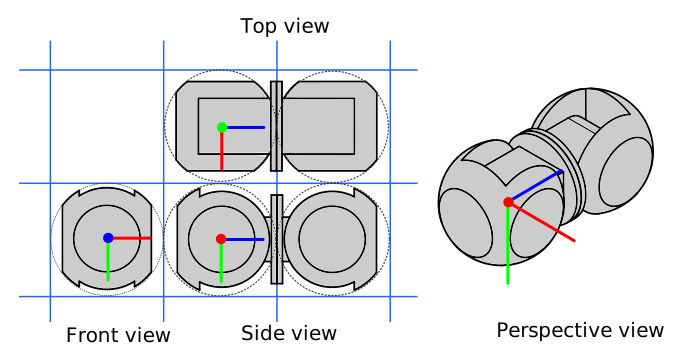
\includegraphics[width=\textwidth]{figures/um_reference.pdf}
    \caption{The universal RoFI module. Blue lines specify the grid, dotted
    lines marks spheres in which the module in inscribed. Note that we show the
    module with the Z axe facing right as it better fits  the page layout. }
    \label{fig:um_reference}
\end{figure}

\begin{figure}[t]
    \centering
    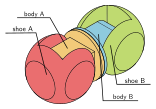
\includegraphics[width=0.7\textwidth]{figures/um_body_parts.pdf}
    \caption{Parts of the universal module.}
    \label{fig:um_body_parts}
\end{figure}

There are 3 degrees of freedom (figure \ref{fig:um_axis}):
\begin{enumerate}
    \item shoe A can rotate against body A along the $\alpha$ axe in a range
    $\langle -90^\circ; +90^\circ\rangle$,
    \item shoe B can rotate against body B along the $\beta$ axe in a range
    $\langle -90^\circ; +90^\circ\rangle$, and
    \item body A can rotate against body B along the $\gamma$ axe in $\langle
    -180^\circ; +180^\circ\rangle$ with an overflow\footnote{First prototypes
    feature a limitation on a number of overflows in one direction on the
    $\gamma$ axe due to technical limitations. }.
\end{enumerate}
The module should be able to provide at least 1.5 $\text{N}\cdot\text{m}$ of
torque for each axe.

\begin{figure}
    \centering
    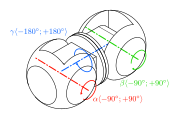
\includegraphics[width=0.7\textwidth]{figures/um_axis.pdf}
    \caption{Degrees of freedom of the universal module. The figure represents
    neutral position of each joint.}
    \label{fig:um_axis}
\end{figure}

There are 3 docks on each shoe -- docks $X+, X-$ and $Z-$. The position of the
docks is captured in figure \ref{fig:um_docks}. The shape descriptor in figure
\ref{fig:um_descriptor} captures the universal module arrangement.

\begin{figure}
    \centering
    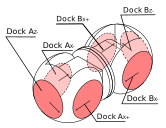
\includegraphics[width=0.7\textwidth]{figures/um_docks.pdf}
    \caption{Docks on the universal module. The arrow on each dock specifies its orientation.}
    \label{fig:um_docks}
\end{figure}

Such a module arrangement is more versatile than to the M-TRAN arrangement.
Addition of the third axe, the $\gamma$ axe, overcomes two limitations of
M-TRAN-like arrangement:
\begin{enumerate*}
    \item given a chain configuration with all joints parallel to each other,
    the system can span only in two dimensions; it cannot expand into the third
    dimension.
    \item Also, given a ring configuration which can roll forward, the M-TRAN
    module cannot steer and only moves forward.
\end{enumerate*}


\section{Universal Module Sensors}

We design the universal module to be rather sensor-impecunious rather than
sensor-rich. There should be various RoFI systems with various sensor needs.
Therefore, we find much useful to implement in the universal module only sensors
that can be beneficial nearly in all systems. The special sensors for concrete
systems should be implemented as separate modules.

There are two types of sensors in each universal module:
\begin{enumerate*}
    \item inertial measurement unit (IMU) and
    \item distance sensors in the middle of each dock.
\end{enumerate*}
The IMU provides a basic notion of the module orientation in the space. Data
from IMU can be used in algorithms to, e.g., determine a common direction in
space among all modules using the Earth's gravitational force. A good solution
for the IMU IC is MPU-9250 \cite{noauthor_mpu-9250_2016} due to broad community
support and all-in-one-package solution (accelerometer, gyroscope, and
magnetometer).

We plan to use the VL53L1X \cite{noauthor_new_2018} time-of-flight distance
sensor in each dock. The sensors allow the universal module to detect obstacles
in front of the module, help to establish correct alignment of two docks when
connecting and can also be used to scan the environment. The scanning of the
environment is performed by moving a shoe and building a depth map. The depth
map can be used as a simple input for computer vision. For example, when the
RoFI system is supposed to climb the stairs, it can measure their geometry by
this procedure.

\section{Intra-module Architecture}

Each universal module is an autonomous unit. A single \emph{control unit}
controls the module. This unit controls all the other components of the module
as can be seen in figure \ref{fig:um_internal}. The unit controls smart
servomotors over a bus built on top UART, docks over SPI bus and directly
controls charging and power management circuits.

\begin{figure}
    \centering
    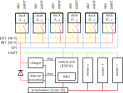
\includegraphics[]{figures/um_internal.pdf}
    \caption{Block diagram of internal architecture of the module.}
    \label{fig:um_internal}
\end{figure}

\subsection{Control Unit}

The control unit is designed to be powered by the ESP32 microcontroller
\cite{noauthor_esp32_2018}. This microcontroller provides enough computational
power, provides rich peripherals including Bluetooth 4 Low Energy and WiFi
802.11 b/g/n, and most importantly, the vendor provides excellent software
support. We are mainly concerned by three aspects of the software support:
\begin{enumerate*}
    \item there is support for modern C/C++ compilers with full support for the
    C++ standard library (including exception handling and concurrency),
    \item the development framework provides POSIX compatible interface, and
    \item there is a vendor maintained port of the lwIP library.
\end{enumerate*}

First two aspects are crucial for easy development of software. From a practical
aspect, the ESP32 is nearly indistinguishable from a desktop POSIX environment
while it still preserves real-time nature and easy access to low-level
peripherals. The POSIX compatibility allow the developers to leverage existing
libraries and port them to the universal module without a significant effort.
The support for lwIP is a benefit as the control unit serves as network
switch (as defined in section \ref{sec:communication}) and therefore, we can
use it. The only necessary part of implementing is the custom device driver for the
docks.

The control unit is not supposed to provide any sensors except the IMU since the
placement of IMU in the robot is not crucial. The distance sensors on the docks
are controlled by a microcontroller on the dock and the control unit.


\subsection{Motors}

We decided to use so-called \emph{smart servomotors} (servos) to power the
universal module. These servos are similar to their hobby counterparts. Just
like the hobby servo, a smart servo is a DC motor with a gearbox combined with a
driver and feedback loop controller in a single compact package. The main
difference between these two is that smart servos provide a digital bus for
sending commands (unlike pulse-width modulation communication used in hobby
servos) and offer several advanced features. The hobby servo can be controlled
only in position mode without any feedback to the control system. The smart
servos usually allow for multiple control modes (torque, speed, and position),
allow continuous rotation and also provide feedback to the control system.
Therefore, the system can detect when the motor reaches a commanded
position or if the motor is overloaded.

The usage of smart servos simplifies both, the mechanical construction and the
control unit, as we can omit motor driver, custom gearing and encoders. In our
design, we use HerkuleX DRS-0101 \cite{noauthor_herkulex_nodate} servos. These
servos are designed to be powered directly from a two cell li-ion accumulator
and provide 1.2 N$\cdot$m of torque at maximal speed one turn per second. The
servos communicate over UART bus, where the control unit serves as a master and
the servos are slaves. The servos can be daisy-chained and therefore, only two
wires are required for the communication. The command set provides means to
perform a synchronized movement.

We choose the DRS-0101 servos for several reasons: they feature slightly smaller
mechanical size compared to the Dynamixel AX-12A \cite{noauthor_dynamixel_2006}
(a comparable servo), they are mechanically compatible with DRS-0201
\cite{noauthor_herkulex_nodate} servos, which feature twice the power. The servo
is also mechanically compatible with Lewansoul LX-16A
\cite{noauthor_lx-16a_2018}, which is a low-cost alternative for possible future
mass production.

\subsection{Power Management}

The module is supposed to be powered from a two cell li-ion accumulator pack.
The motors can directly operate from the accumulator at their rated voltage and
can drain sufficient current. The control unit is also powered from the
accumulator.

The internal connection of power rails is captured in figure
\ref{fig:um_internal}. There is a charger circuit to allow for charging from the
INT line. The charger is controlled by the control unit -- it can be either
disabled or it can charge the accumulator with given power limit. There is also
a step-up convertor used to source power to other modules. The used step-up
convertors must be parallelizable (denoted by a diode in the block diagram). The
step-up module is also controlled by the control unit and can be disabled when
not needed.

Provided this power sharing setup, the module can operate in four modes:

\paragraph{Self-powered mode} The module runs on its own accumulator (charger is
disabled and convertor is disabled).

\paragraph{Power sourcing mode} The module provides energy to the network
(charger is disabled and convertor is enabled).

\paragraph{Power draining mode} The module charges its accumulator and drains
power from other modules.

\paragraph{Survivor mode} The module disables motors, disables converter and
limits the charging power roughly to cover energy consumption of the control
module. Therefore, no charging occurs and the charger is acts as a step-down
converter for the control unit.

The communication in the RoFI platform requires an activity from the control
unit as it routes packets between the docks. If a module shuts down due to
discharged accumulator, there cannot be any communication across the module.
Dead module might lead to a separation of the system into two independent
networks in some configurations. Charging the dead module might not be strategic
in many cases. Therefore, survivor mode can be applied to keep the communication
going without waisting power on charging the dead module.
